\documentclass[11pt,a4paper]{article}
\usepackage[T1]{fontenc}
\usepackage[utf8]{inputenc}
\usepackage{babel}
\babelprovide[main,import]{italian}
\usepackage[margin=25mm]{geometry}
\usepackage{lmodern}
\usepackage{microtype}
\usepackage{amsmath,amssymb}
\usepackage{graphicx}
\usepackage{booktabs}
\usepackage{subcaption}
\usepackage[section]{placeins}
\usepackage[hidelinks]{hyperref}
\IfFileExists{../analysis/defense_metrics.csv}{\graphicspath{{../}}}{\graphicspath{{./}}}
\captionsetup{font=small,labelfont=bf}
\setlength{\emergencystretch}{2em}
\setlength{\tabcolsep}{5pt}
\renewcommand{\arraystretch}{1.12}
\title{Explainability delle predizioni di FOLD sul traffico ODoH\\
\large Analisi closed-world, defense e open-world}
\author{}
\date{}
\begin{document}
\maketitle

\section{Introduzione}
Il lavoro riguarda l'aggiunta di explainability a FOLD. L'obiettivo è capire quali informazioni contribuiscono alle sue predizioni e rendere più leggibile il comportamento del modello sulle tracce analizzate.

Come primo passo ho analizzato la Random Forest con TreeSHAP, per osservare il contributo delle singole feature alla probabilità del sito target. Questa analisi permette di capire la previsione della RF, ma non spiega ancora la decisione finale di FOLD. Per questo ho poi implementato una spiegazione end-to-end, che parte dalla traccia e ricalcola tutti gli input prima di valutare l'output finale.

Infine ho esteso l'analisi alle configurazioni con defense e allo scenario open-world con background traffic. Ho affiancato le spiegazioni alle metriche di classificazione, per osservare sia le performance complessive sia i contributi ottenuti sui campioni selezionati.

\section{Metodologia di explainability}
\subsection{TreeSHAP sulla Random Forest}
La Random Forest utilizza 97 feature: 33 statistiche aggregate e 64 conteggi dell'istogramma delle dimensioni dei pacchetti. Per spiegare la RF ho utilizzato TreeSHAP, che assegna a ciascuna feature un contributo alla probabilità della classe target rispetto a un riferimento. Un contributo positivo aumenta questa probabilità; uno negativo la diminuisce.

I campioni da spiegare sono tracce del test set sulle quali vogliamo capire la decisione del modello. Le reference sono invece tracce di training utilizzate per definire il riferimento rispetto al quale vengono calcolati i contributi. In questo contesto, una reference non indica necessariamente traffico background. La classe target è la classe di cui spieghiamo la probabilità: nella baseline ho scelto la classe 8, \texttt{instagram.com}, utilizzando 16 tracce Instagram di test e 64 reference di training.

Una spiegazione locale riguarda una singola traccia e mostra quali feature aumentano o diminuiscono la probabilità del target. Aggregando più spiegazioni locali possiamo osservare quali feature hanno mediamente contributi più grandi nel cohort analizzato. Nei grafici globali uso la media dei valori assoluti: questa misura indica la magnitudine del contributo, mentre per conoscerne la direzione occorre considerare il segno.

TreeSHAP spiega la Random Forest, non automaticamente la previsione finale di FOLD. Questa analisi è stata quindi un primo livello di explainability e un modo per verificare il funzionamento della pipeline prima di passare alla spiegazione completa di FOLD.

\subsection{Explainability end-to-end di FOLD}
Gli input utilizzati da FOLD derivano tutti dalla stessa traccia ODoH. Non sarebbe corretto modificare soltanto la rappresentazione sequenziale lasciando inalterate le feature della Random Forest o le sue probabilità: i diversi input non rappresenterebbero più la stessa traccia e la spiegazione riguarderebbe una combinazione incoerente di informazioni.

Per questo motivo ho implementato un predictor end-to-end. Il predictor riceve una traccia, applica l'Encoder e il preprocessing, ricava le feature della RF e calcola le probabilità con la Random Forest finale. Ricostruisce poi gli input sequenziali e statistici di FOLD e valuta il modello usando anche le probabilità RF appena ottenute. Lo schema seguito è:
\begin{center}
\begin{tabular}{c}
Traccia perturbata \\
$\downarrow$ \\
Encoder / preprocessing \\
$\downarrow$ \\
Feature Random Forest \\
$\downarrow$ \\
Random Forest finale \\
$\downarrow$ \\
Probabilità RF \\
$\downarrow$ \\
Input sequenziali e statistici FOLD \\
$\downarrow$ \\
FOLD \\
$\downarrow$ \\
Probabilità della classe target
\end{tabular}
\end{center}
Ogni volta che l'explainer crea una traccia ibrida, tutti gli input vengono ricalcolati da quella stessa traccia. In questo modo la spiegazione comprende anche le variazioni delle informazioni fornite dalla RF. L'Encoder e i modelli già addestrati vengono usati per la previsione: durante SHAP il modello non viene riaddestrato. Per l'analisi multiclass spiego \texttt{multi\_output}, cioè l'output finale multiclass di FOLD, selezionando la probabilità della classe target.

\subsection{Valori Shapley esatti per gruppi}
Per spiegare l'output finale ho diviso ogni traccia in quattro gruppi consecutivi e bilanciati di risoluzioni complete, indicati con G1, G2, G3 e G4. G1 contiene la parte iniziale secondo l'ordine delle risoluzioni e G4 quella finale. Sono blocchi relativi alla lunghezza della traccia, non quattro intervalli di uguale durata temporale. Anche ogni traccia reference viene suddivisa nello stesso modo.

Per valutare il contributo di un gruppo, l'explainer costruisce tracce ibride: mantiene alcuni gruppi del campione da spiegare e sostituisce gli altri con i gruppi corrispondenti di una traccia reference. Ogni combinazione di gruppi mantenuti, chiamata coalizione, viene valutata con il predictor end-to-end. Il procedimento viene ripetuto sulle reference e le probabilità ottenute vengono mediate.

Il valore Shapley di un gruppo riassume quanto cambia la probabilità quando quel gruppo viene aggiunto alle diverse combinazioni degli altri. Con quattro gruppi ci sono soltanto $2^4=16$ coalizioni: è quindi possibile valutarle tutte e calcolare il valore esatto per questo raggruppamento e per le reference scelte. La coalizione vuota corrisponde alle reference e quella completa alla traccia originale. Indicando con $N=\{1,2,3,4\}$ l'insieme dei gruppi e con $v_x(S)$ la probabilità media per la coalizione $S$, il contributo del gruppo $g$ è:
\begin{equation}
\phi_g(x)=\sum_{S\subseteq N\setminus\{g\}}
\frac{|S|!\,(4-|S|-1)!}{4!}
\left[v_x(S\cup\{g\})-v_x(S)\right].
\label{eq:shapley}
\end{equation}
La formula viene applicata ai quattro gruppi. Nella baseline ho spiegato 15 tracce Instagram, con target class 8, quattro gruppi, 16 reference di training e seed 0. I contributi con segno descrivono la differenza tra la probabilità della traccia e la probabilità media delle reference; la media dei valori assoluti permette di confrontare le magnitudini dei quattro gruppi sul cohort.

Le tracce ibride sono create appositamente dall'explainer per osservare come cambia la predizione e non rappresentano necessariamente traffico reale. I gruppi indicano una posizione relativa nella traccia, non quattro fasi temporali fisiche. I valori descrivono il comportamento del modello rispetto alle reference scelte e non dimostrano una relazione causale nel traffico reale.

\section{Configurazione sperimentale}
\subsection{Dataset e configurazioni}
Il dataset monitored, \texttt{data/odoh\_traces.csv}, contiene 100 siti, 2.834 tracce di caricamento di pagina e 54.155 righe di risoluzioni ODoH. Ogni riga rappresenta una risoluzione. 

Lo split assegna il 65\% delle tracce al training, il 10\% alla validazione e il 25\% al test: rispettivamente 1.842, 283 e 709 tracce monitored. Ho eseguito una sola repetition per configurazione. La Tabella~\ref{tab:campaign} riassume la baseline, le cinque configurazioni open-world e le venti configurazioni defense.

\begin{table}[htbp]
\centering\small
\caption{Le 26 configurazioni sperimentali. Le defense sono valutate senza background; le configurazioni open-world senza defense.}
\label{tab:campaign}
\begin{tabular}{llr}
\toprule
Scenario & Rapporto background o intensità defense & Configurazioni \\
\midrule
Baseline & Senza background e defense & 1 \\
Open-world & Background 30/40/50/60/70\% & 5 \\
Padding & Intensità 10/30/50/70/100\% & 5 \\
Dummy & Intensità 10/30/50/70/100\% & 5 \\
Fragmentation & Intensità 10/30/50/70/100\% & 5 \\
Combined & Ogni meccanismo al 10/30/50/70/100\% & 5 \\
\midrule
Totale & & 26 \\
\bottomrule
\end{tabular}
\end{table}

Il padding modifica le dimensioni, dummy aggiunge record e fragmentation suddivide i payload che soddisfano le condizioni previste. L'intensità indica la probabilità di applicazione del meccanismo. Combined applica tutti e tre i meccanismi alla stessa intensità. Le defense sono applicate a training, validazione e test, addestrando i modelli per ciascuna configurazione, senza background.

Nello scenario open-world il background proviene da un insieme sintetico comune. Il rapporto indica la frazione prevista di background nel totale delle tracce; queste configurazioni non includono defense.

\subsection{Campioni utilizzati per le spiegazioni}
Le metriche di performance sono calcolate sull'intero test set, mentre le spiegazioni riguardano i campioni della Tabella~\ref{tab:cohorts}. Le stesse 15 tracce Instagram vengono utilizzate per la baseline FOLD, le defense, l'analisi multiclass open-world e il cohort monitored dell'analisi binary. Per TreeSHAP uso un insieme separato di 16 tracce Instagram.

\begin{table}[htbp]
\centering\small
\caption{Campioni spiegati e reference di training. Per FOLD si usano quattro gruppi di risoluzioni; per la RF, 97 feature.}
\label{tab:cohorts}
\begin{tabular}{p{0.22\linewidth}p{0.27\linewidth}p{0.23\linewidth}p{0.14\linewidth}}
\toprule
Analisi & Campioni di test & Reference & Unità \\
\midrule
Baseline RF & 16 Instagram & 64 monitored & 97 feature \\
Baseline FOLD & 15 Instagram & 16 monitored & 4 gruppi \\
FOLD con defense & Stesse 15 Instagram & 16 monitored & 4 gruppi \\
Open-world multiclass & Stesse 15 Instagram & 16 monitored & 4 gruppi \\
Open-world binary & 15 monitored + 15 background & 8 + 8 miste & 4 gruppi \\
\bottomrule
\end{tabular}
\end{table}

\subsection{Metriche}
L'accuracy è la frazione di predizioni corrette; nello scenario open-world comprende anche il corretto riconoscimento del background. La macro-F1 è la media degli F1 delle classi monitored: il background contribuisce come esempio negativo, ma non è incluso come classe nella media.

Il TPR indica la quota di tracce monitored riconosciute come tali. Il FPR indica la quota di tracce background erroneamente riconosciute come monitored. Entrambi sono calcolati con soglia $>0.5$. La ROC AUC riassume la capacità di distinguere monitored e background considerando tutte le soglie. Per FOLD il punteggio è l'output binary; per la RF si usa la massima probabilità multiclass riscalata. Le metriche sono espresse tra 0 e 1.

\section{Risultati closed-world}
\subsection{Performance}
Nella baseline, senza defense e background, la RF raggiunge accuracy 0.9887 e macro-F1 0.9886; FOLD raggiunge accuracy 0.9873 e macro-F1 0.9832. Entrambi ottengono quindi performance elevate. I valori arrotondati sono riportati nella Tabella~\ref{tab:defense-performance}.

\subsection{TreeSHAP RF}
La Figura~\ref{fig:baseline-rf} mostra l'importanza delle feature per la probabilità della classe 8. Le feature con i maggiori contributi medi assoluti sono la deviazione standard delle dimensioni dei pacchetti (0.0453), la dimensione media (0.0403) e la dimensione media delle risposte del target (0.0397). Tra le feature principali compaiono anche conteggi dell'istogramma delle dimensioni e statistiche delle dimensioni per ruolo. L'ultima barra somma i contributi delle altre 83 feature e va letta come un'aggregazione.

\begin{figure}[htbp]
\centering
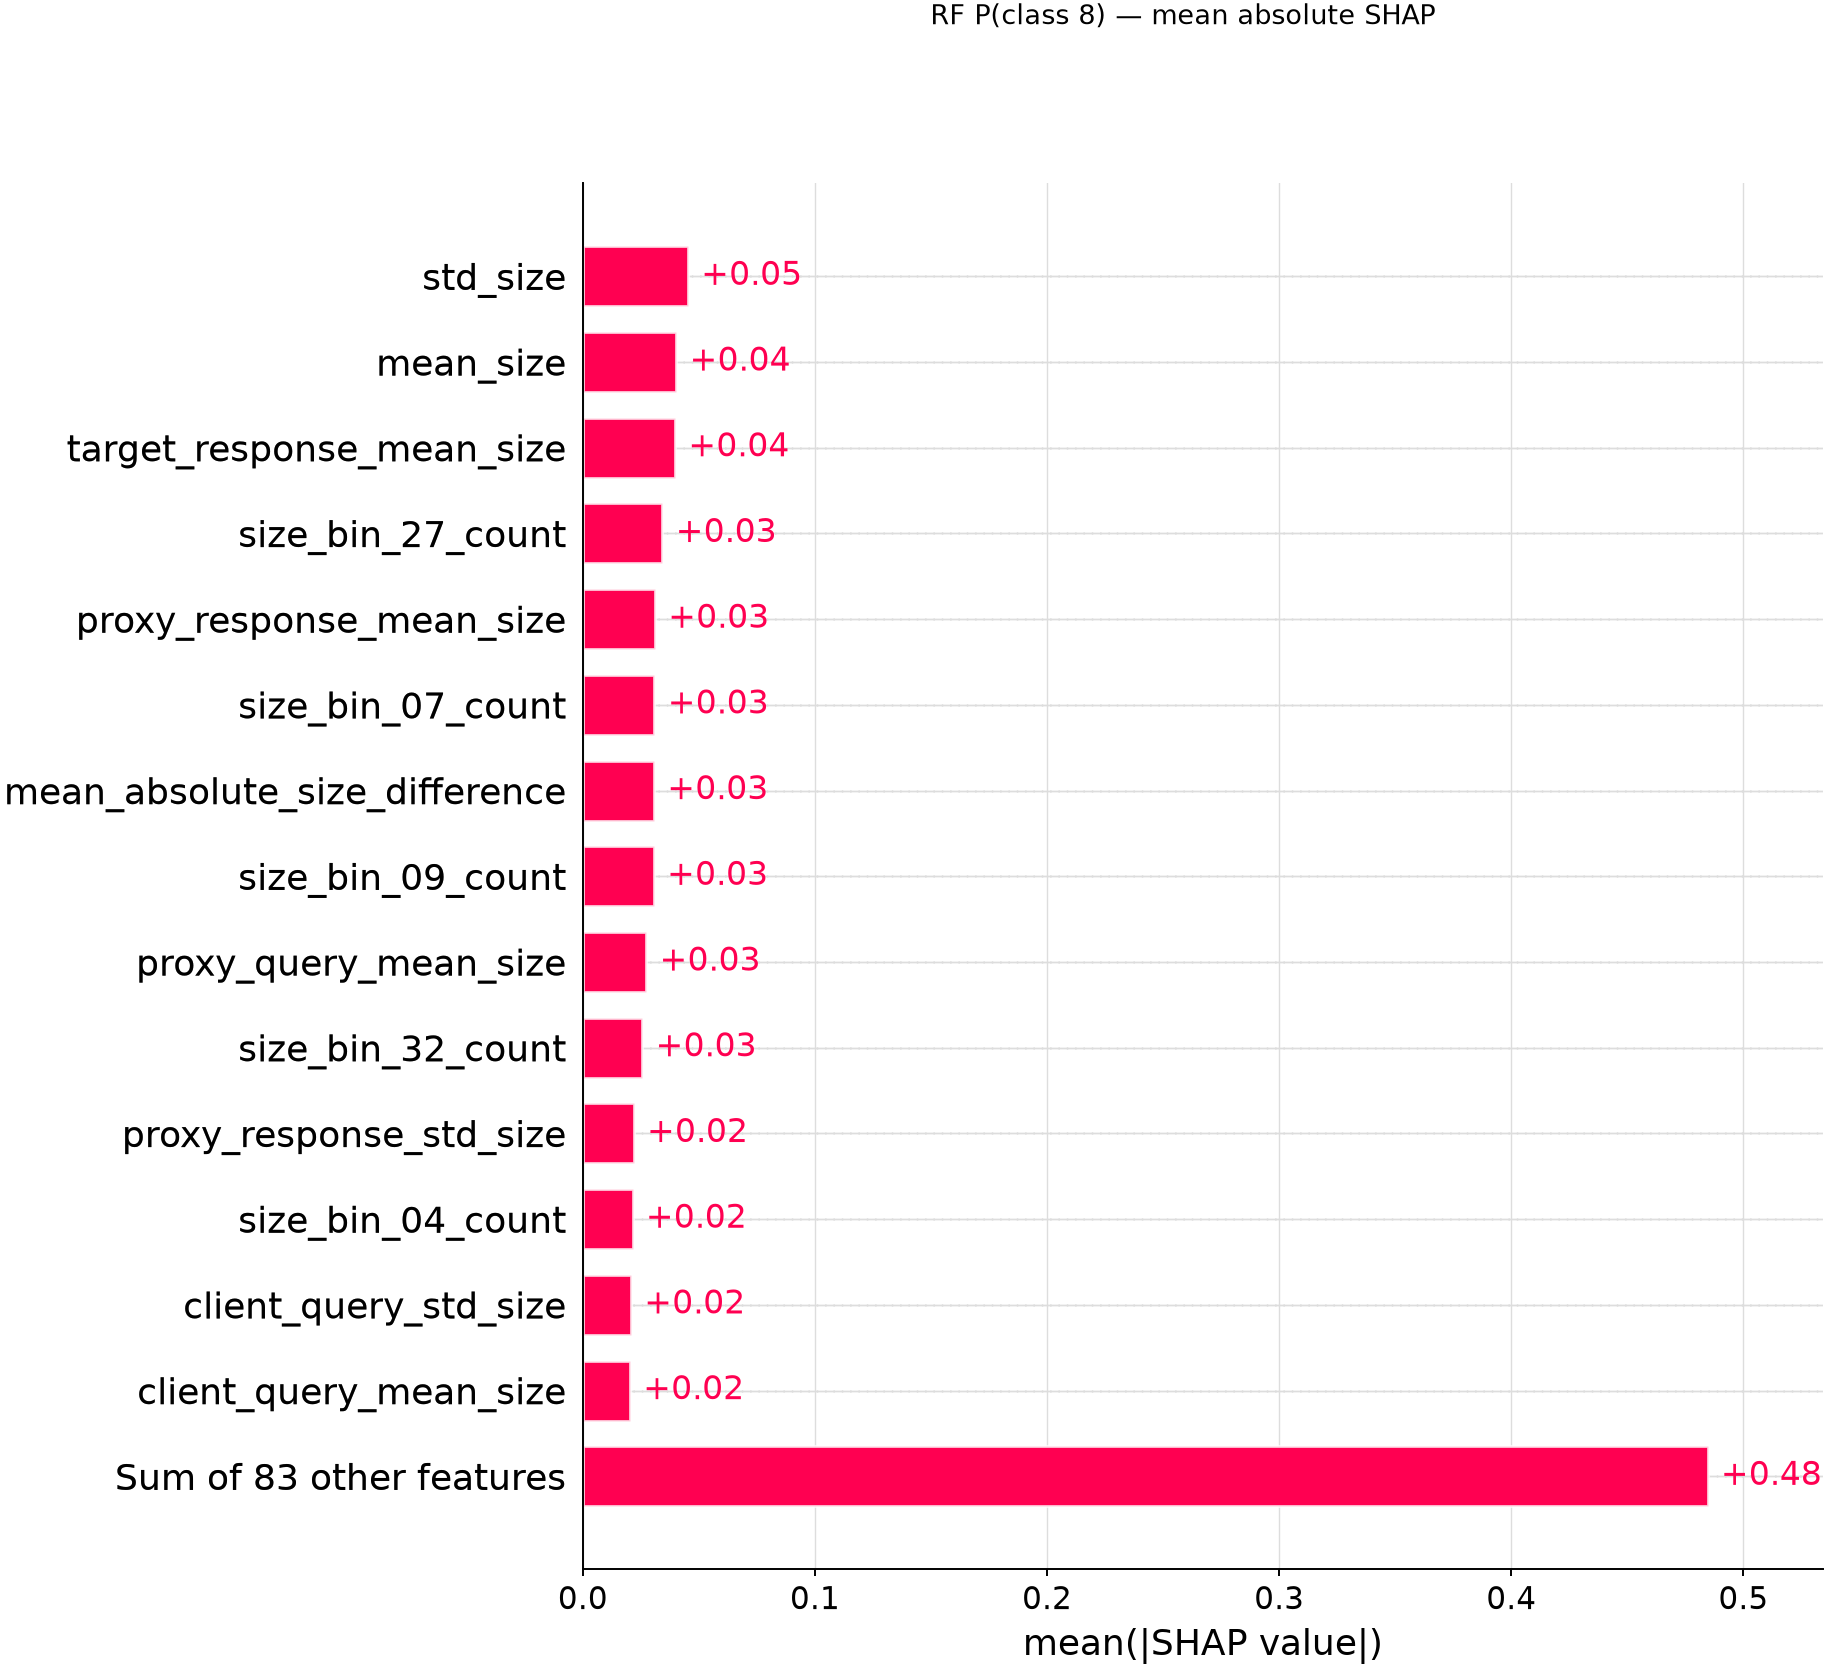
\includegraphics[width=0.78\linewidth]{explanations/baseline/rf_instagram/rf_class_008_bar.png}
\caption{TreeSHAP della RF per $P(\mathrm{Instagram})$: 16 tracce di test e 64 reference di training. Le barre mostrano i contributi medi assoluti; l'ultima riunisce le altre 83 feature.}
\label{fig:baseline-rf}
\end{figure}

\subsection{Grouped Shapley FOLD}
Nelle tracce Instagram selezionate, il primo blocco relativo presenta mediamente il contributo assoluto maggiore, seguito da G2. I valori per G1--G4 sono rispettivamente 0.2950, 0.2146, 0.1654 e 0.1687: G3 e G4 risultano più bassi, ma mantengono contributi apprezzabili (Figura~\ref{fig:baseline-fold}).

I contributi dei gruppi nella baseline sono positivi. La probabilità media Instagram è 0.8451, rispetto a una probabilità media delle reference di 0.0014. Questa osservazione riguarda il cohort Instagram analizzato. Le magnitudini RF e FOLD non sono direttamente confrontabili, perché le due analisi spiegano modelli diversi con feature o gruppi, reference e campioni differenti.

\begin{figure}[htbp]
\centering
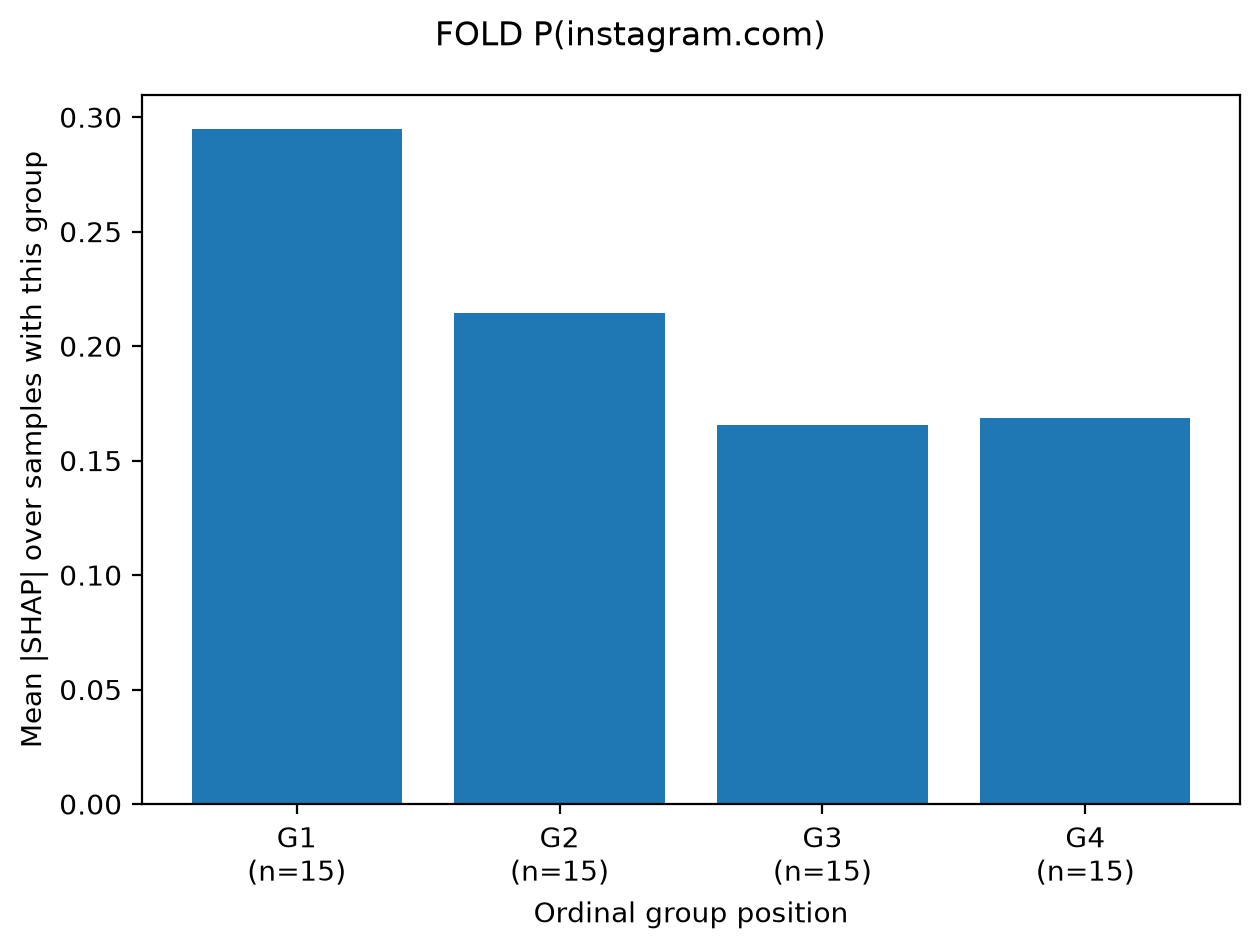
\includegraphics[width=0.82\linewidth]{explanations/baseline/fold_instagram/fold_class_008_bar.png}
\caption{Contributi medi assoluti grouped Shapley di FOLD per $P(\mathrm{Instagram})$: 15 tracce di test, 16 reference e quattro gruppi consecutivi di risoluzioni.}
\label{fig:baseline-fold}
\end{figure}

\section{Risultati con defense}
\subsection{Performance}
La Tabella~\ref{tab:defense-performance} riporta tutte le 20 configurazioni e la baseline per RF e FOLD; la Figura~\ref{fig:defense-performance} mostra l'accuracy di FOLD. Il padding riduce soprattutto le performance alle intensità più alte: a 1.00 FOLD raggiunge accuracy 0.578 e macro-F1 0.571. Con dummy l'accuracy rimane elevata, tra 0.979 e 0.990, con variazioni non monotone.

Fragmentation presenta una degradazione più moderata rispetto a padding e combined: l'accuracy FOLD scende a 0.928 a intensità 0.70 e risale a 0.941 a 1.00. Combined mostra una forte riduzione alle intensità intermedie e alte, con il minimo di accuracy 0.547 a 0.70 e un recupero a 0.732 a 1.00. Questo recupero è quanto osservato nella singola run.

\begin{table}[htbp]
\centering\small
\caption{Performance della baseline e delle 20 configurazioni defense, senza background. Accuracy e macro-F1 sono calcolate su tutto il test set.}
\label{tab:defense-performance}
\begin{tabular}{lrrrrr}
\toprule
Defense & Intensità & RF accuracy & RF macro-F1 & FOLD accuracy & FOLD macro-F1 \\
\midrule
Baseline & 0.00 & 0.989 & 0.989 & 0.987 & 0.983 \\
Padding & 0.10 & 0.979 & 0.976 & 0.979 & 0.980 \\
Padding & 0.30 & 0.953 & 0.952 & 0.962 & 0.959 \\
Padding & 0.50 & 0.890 & 0.891 & 0.904 & 0.901 \\
Padding & 0.70 & 0.745 & 0.746 & 0.756 & 0.758 \\
Padding & 1.00 & 0.477 & 0.461 & 0.578 & 0.571 \\
Dummy & 0.10 & 0.983 & 0.978 & 0.990 & 0.989 \\
Dummy & 0.30 & 0.976 & 0.969 & 0.983 & 0.980 \\
Dummy & 0.50 & 0.975 & 0.969 & 0.980 & 0.976 \\
Dummy & 0.70 & 0.972 & 0.965 & 0.990 & 0.988 \\
Dummy & 1.00 & 0.970 & 0.966 & 0.979 & 0.974 \\
Fragmentation & 0.10 & 0.979 & 0.974 & 0.987 & 0.987 \\
Fragmentation & 0.30 & 0.963 & 0.957 & 0.966 & 0.961 \\
Fragmentation & 0.50 & 0.938 & 0.933 & 0.953 & 0.952 \\
Fragmentation & 0.70 & 0.922 & 0.916 & 0.928 & 0.926 \\
Fragmentation & 1.00 & 0.925 & 0.920 & 0.941 & 0.939 \\
Combined & 0.10 & 0.959 & 0.955 & 0.959 & 0.958 \\
Combined & 0.30 & 0.839 & 0.840 & 0.839 & 0.840 \\
Combined & 0.50 & 0.643 & 0.632 & 0.674 & 0.678 \\
Combined & 0.70 & 0.496 & 0.477 & 0.547 & 0.528 \\
Combined & 1.00 & 0.654 & 0.640 & 0.732 & 0.729 \\
\bottomrule
\end{tabular}
\end{table}

\begin{figure}[htbp]
\centering
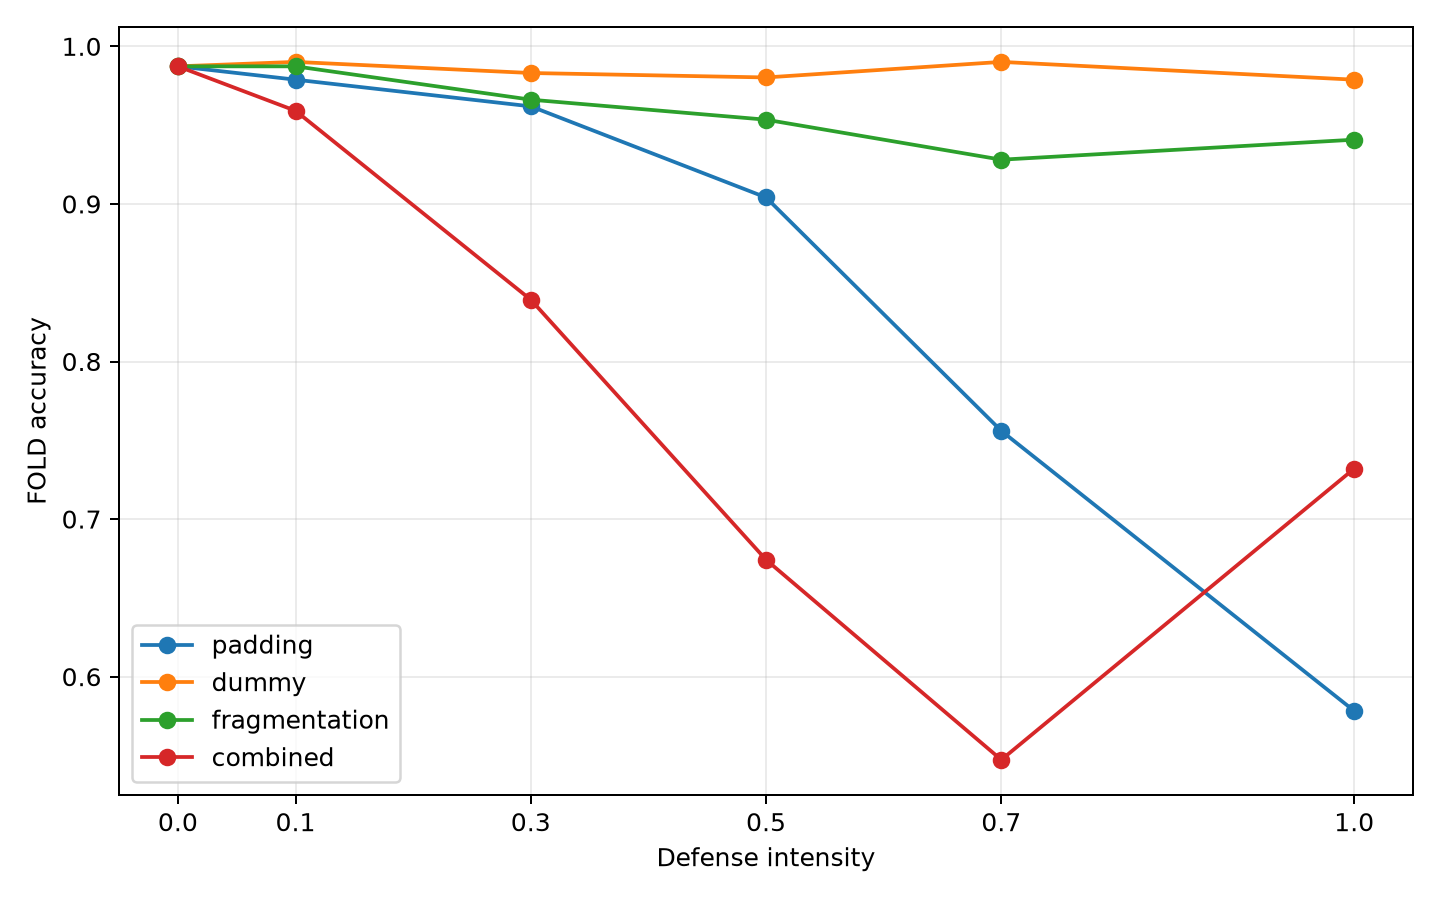
\includegraphics[width=0.9\linewidth]{analysis/defense_fold_accuracy.png}
\caption{Accuracy di FOLD per le quattro defense, senza background, al variare dell'intensità.}
\label{fig:defense-performance}
\end{figure}

\subsection{Probabilità Instagram e contributi dei gruppi}
La Figura~\ref{fig:defense-xai} mostra i contributi dei quattro gruppi per ogni defense, mentre la Figura~\ref{fig:defense-probability} riporta la probabilità media Instagram sulle stesse 15 tracce. La Tabella~\ref{tab:defense-xai} in appendice contiene tutti i valori.

\paragraph{Padding.}
Alle intensità più alte diminuiscono sia la probabilità Instagram sia le attribuzioni (Figura~\ref{fig:defense-padding}). A 1.00 la probabilità media è 0.0262 e i contributi medi assoluti sono compresi tra 0.0041 e 0.0078. Alle intensità basse l'andamento è diverso: a 0.10 la probabilità è 0.9250, superiore alla baseline 0.8451.

\paragraph{Dummy.}
I contributi rimangono relativamente consistenti e G1 mantiene la magnitudine maggiore a tutte le intensità (Figura~\ref{fig:defense-dummy}). La probabilità media Instagram varia tra 0.7965 e 0.9137, senza un andamento monotono. Rispetto alle intensità alte di padding e combined, le attribuzioni rimangono su valori più vicini alla baseline.

\paragraph{Fragmentation.}
G1 rimane il gruppo con il contributo medio assoluto maggiore, ma la distanza dagli altri gruppi si riduce (Figura~\ref{fig:defense-fragmentation}). A 1.00 G1 vale 0.2362, mentre G3 e G4 valgono 0.1963 e 0.2074, superiori ai rispettivi valori di baseline. La probabilità Instagram è 0.8373 a 1.00; il minimo osservato è 0.6807 a 0.50.

\paragraph{Combined.}
A 0.10 G4 e G3 superano G1 e G2 (Figura~\ref{fig:defense-combined}), con probabilità media 0.8410. A 0.50 e 0.70 la probabilità scende a 0.0659 e 0.0393 e tutti i contributi si riducono molto. A 1.00 si osserva un recupero della probabilità, pari a 0.2256, e delle attribuzioni, che restano inferiori alla baseline.

\begin{figure}[htbp]
\centering
\begin{subfigure}{0.49\linewidth}
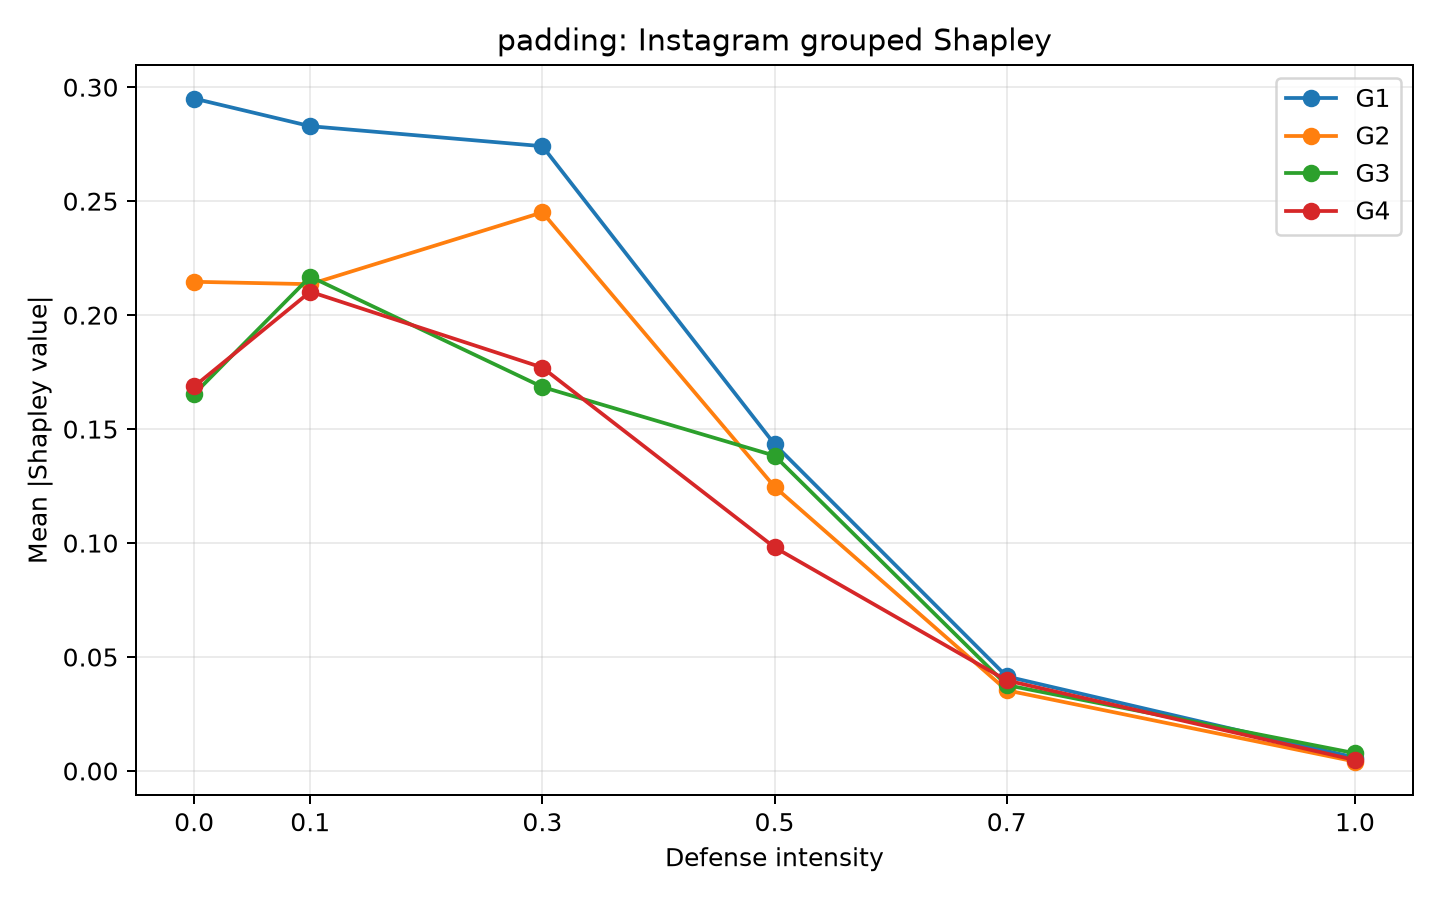
\includegraphics[width=\linewidth]{analysis/defense_padding_mean_abs_phi.png}
\caption{Padding.}\label{fig:defense-padding}
\end{subfigure}\hfill
\begin{subfigure}{0.49\linewidth}
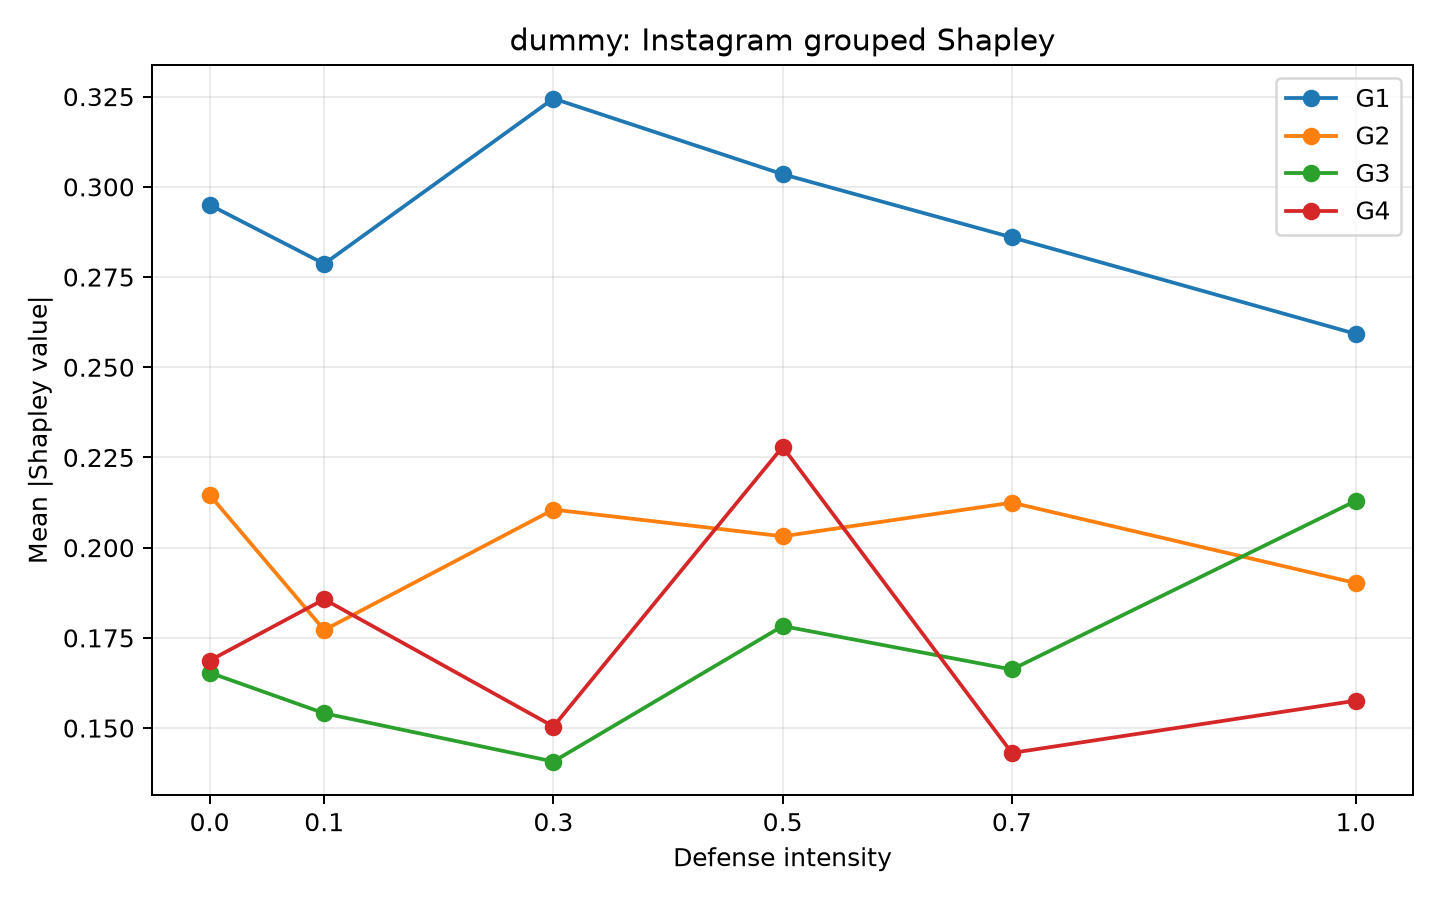
\includegraphics[width=\linewidth]{analysis/defense_dummy_mean_abs_phi.png}
\caption{Dummy.}\label{fig:defense-dummy}
\end{subfigure}
\par\medskip
\begin{subfigure}{0.49\linewidth}
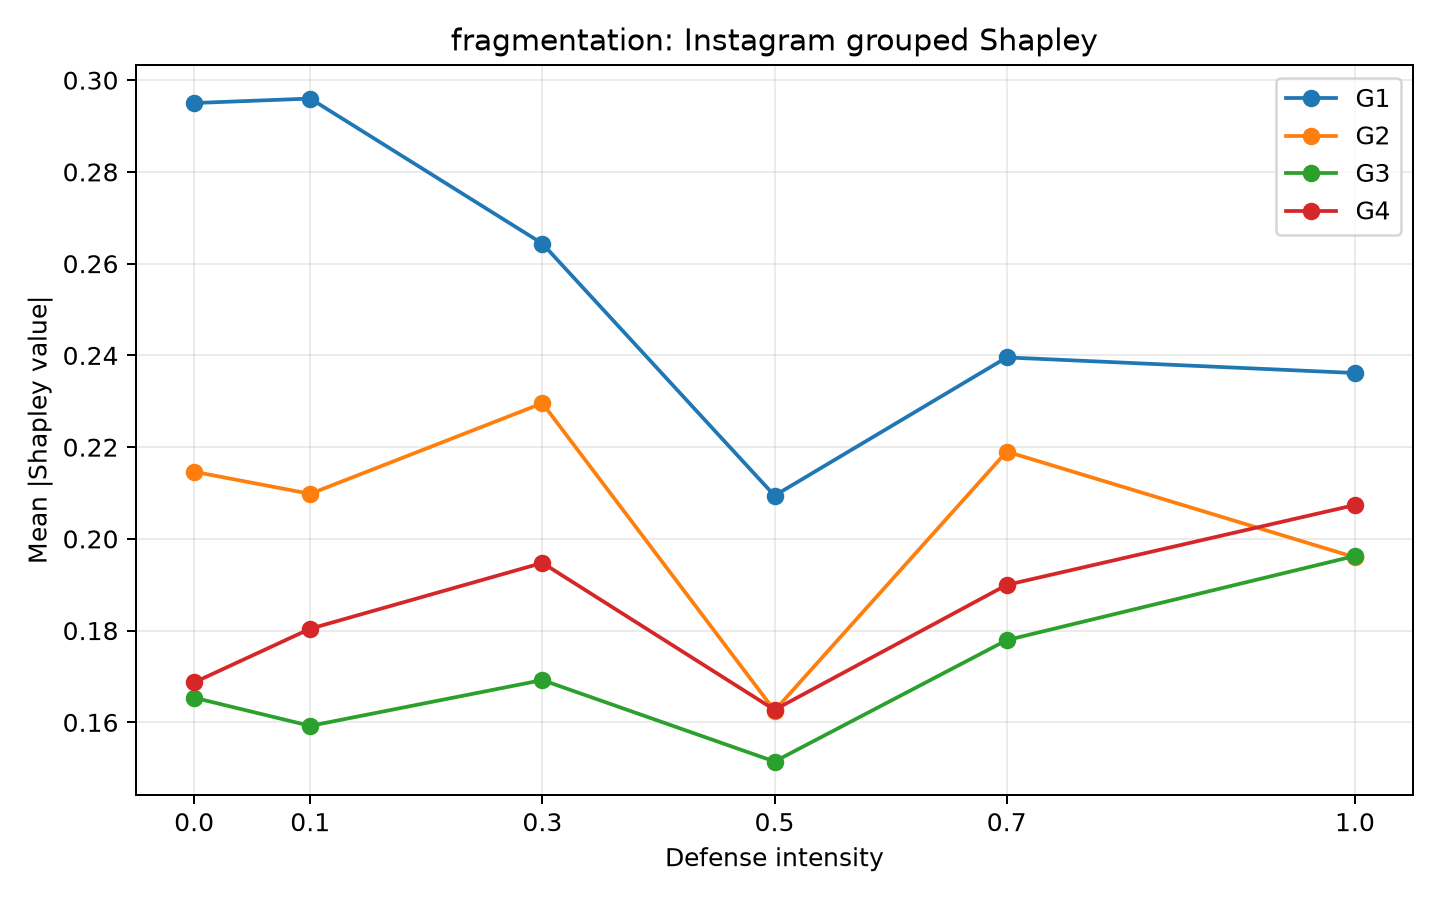
\includegraphics[width=\linewidth]{analysis/defense_fragmentation_mean_abs_phi.png}
\caption{Fragmentation.}\label{fig:defense-fragmentation}
\end{subfigure}\hfill
\begin{subfigure}{0.49\linewidth}
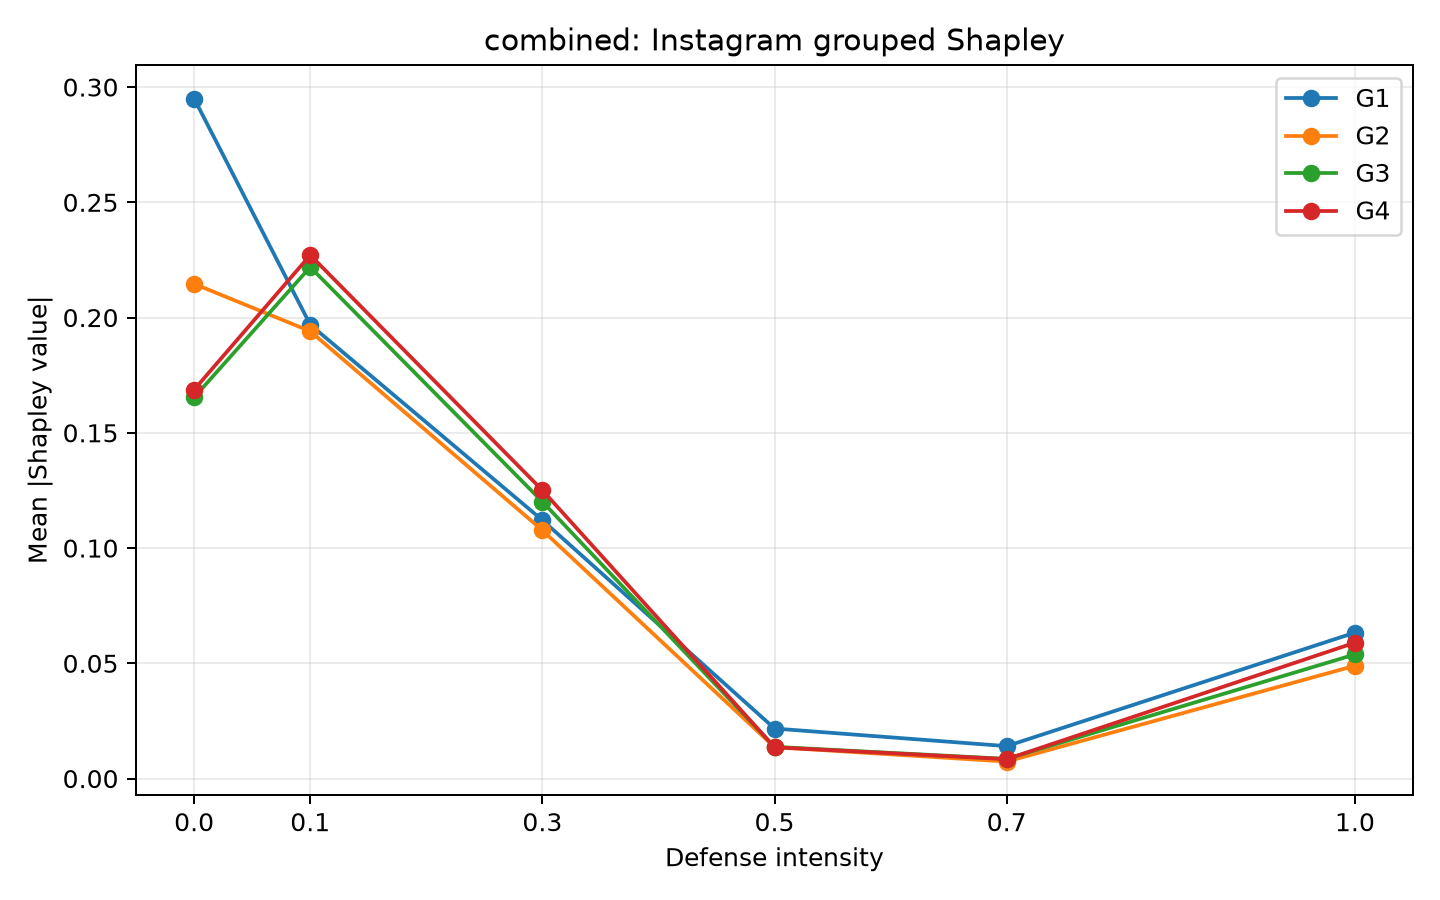
\includegraphics[width=\linewidth]{analysis/defense_combined_mean_abs_phi.png}
\caption{Combined.}\label{fig:defense-combined}
\end{subfigure}
\caption{Contributi medi assoluti di FOLD sulle stesse 15 tracce Instagram per le quattro defense. L'intensità zero indica la baseline. I pannelli hanno scale verticali diverse.}
\label{fig:defense-xai}
\end{figure}

\begin{figure}[htbp]
\centering
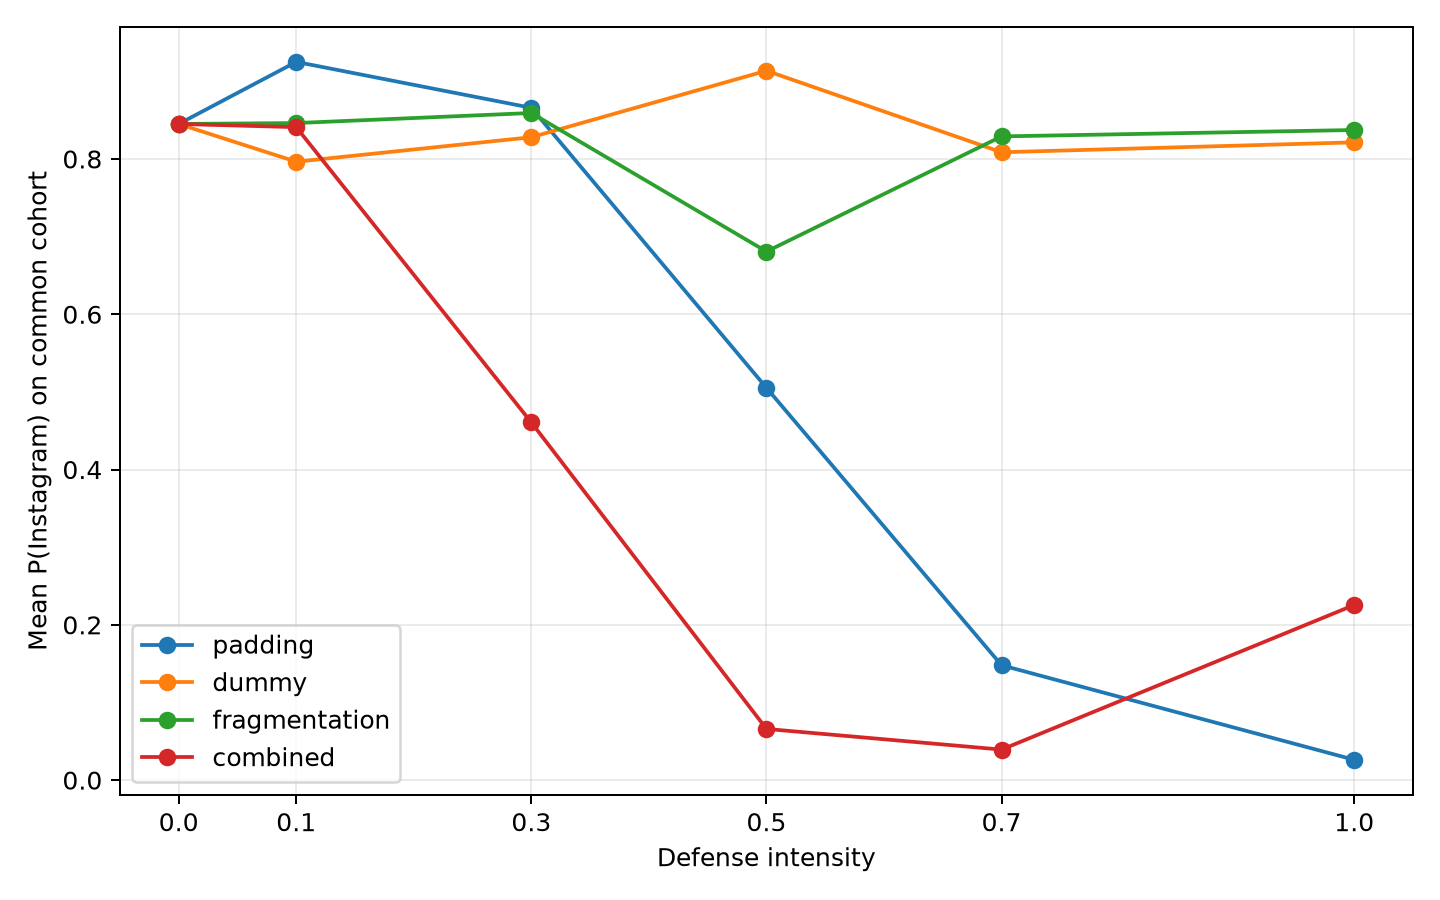
\includegraphics[width=0.9\linewidth]{analysis/defense_instagram_mean_probability.png}
\caption{Probabilità media Instagram assegnata da FOLD al cohort selezionato, al variare della defense e dell'intensità.}
\label{fig:defense-probability}
\end{figure}

\section{Risultati open-world}
\subsection{Open-world: approccio di explainability}
Nel closed-world e nell'analisi multiclass open-world spiego \texttt{multi\_output}, cioè la probabilità assegnata al sito target, in questo caso $P(\mathrm{Instagram})$. Nello scenario open-world è disponibile anche \texttt{binary\_output}$=P(\mathrm{monitored})$, che risponde a una domanda diversa: la traccia appartiene a uno dei siti monitorati oppure al background?

Per questo ho eseguito due analisi. La spiegazione multiclass permette di osservare come cambiano i contributi alla probabilità Instagram quando aumenta la quota di background. La spiegazione binary permette invece di capire quali gruppi spingono la decisione verso monitored oppure verso background. Entrambe utilizzano il predictor end-to-end e lo stesso raggruppamento G1--G4.

Per la binary ho spiegato 15 campioni monitored e 15 campioni background per rapporto, usando 8 reference monitored e 8 reference background di training. Le 16 reference sono comuni ai cinque rapporti. Un valore $\phi$ positivo aumenta $P(\mathrm{monitored})$ rispetto al riferimento; un valore negativo la diminuisce e spinge quindi la decisione verso background.

\subsection{Performance}
Le Tabelle~\ref{tab:open-performance} e~\ref{tab:open-detection} riportano i risultati dei cinque rapporti di background. FOLD ha accuracy, TPR e ROC AUC maggiori della RF in tutti i rapporti. La macro-F1 è maggiore a 0.40, 0.50 e 0.60, ma inferiore a 0.30 e 0.70.

Il FPR di FOLD è maggiore a 0.30, 0.40 e 0.50, inferiore a 0.60 e uguale a quello della RF a 0.70 (0.011487 prima dell'arrotondamento). A 30\% di background FOLD riconosce una quota maggiore di traffico monitored, ma presenta anche un FPR maggiore della RF: TPR/FPR sono 0.984/0.053 per FOLD e 0.955/0.013 per RF. Macro-F1 e FPR non mostrano quindi lo stesso vantaggio in tutti i rapporti. La Figura~\ref{fig:open-performance} riassume accuracy (Figura~\ref{fig:open-accuracy}) e AUC (Figura~\ref{fig:open-auc}).

\begin{table}[htbp]
\centering\small
\caption{Performance open-world nei cinque rapporti di background. L'accuracy include il riconoscimento del background; la macro-F1 riguarda i siti monitored.}
\label{tab:open-performance}
\begin{tabular}{rrrrr}
\toprule
Background & RF accuracy & RF macro-F1 & FOLD accuracy & FOLD macro-F1 \\
\midrule
0.30 & 0.963 & 0.969 & 0.966 & 0.967 \\
0.40 & 0.969 & 0.969 & 0.978 & 0.978 \\
0.50 & 0.968 & 0.965 & 0.976 & 0.969 \\
0.60 & 0.972 & 0.963 & 0.983 & 0.970 \\
0.70 & 0.978 & 0.961 & 0.982 & 0.959 \\
\bottomrule
\end{tabular}
\end{table}

\begin{table}[htbp]
\centering\small
\caption{Riconoscimento del traffico monitored nello scenario open-world. TPR e FPR usano la soglia $>0.5$; ROC AUC considera tutte le soglie.}
\label{tab:open-detection}
\begin{tabular}{rrrrrrr}
\toprule
Background & RF TPR & RF FPR & RF AUC & FOLD TPR & FOLD FPR & FOLD AUC \\
\midrule
0.30 & 0.955 & 0.013 & 0.992 & 0.984 & 0.053 & 0.995 \\
0.40 & 0.955 & 0.008 & 0.993 & 0.989 & 0.025 & 0.998 \\
0.50 & 0.955 & 0.018 & 0.991 & 0.984 & 0.021 & 0.998 \\
0.60 & 0.955 & 0.015 & 0.992 & 0.982 & 0.009 & 0.999 \\
0.70 & 0.955 & 0.011 & 0.992 & 0.979 & 0.011 & 0.996 \\
\bottomrule
\end{tabular}
\end{table}

\begin{figure}[htbp]
\centering
\begin{subfigure}{0.49\linewidth}
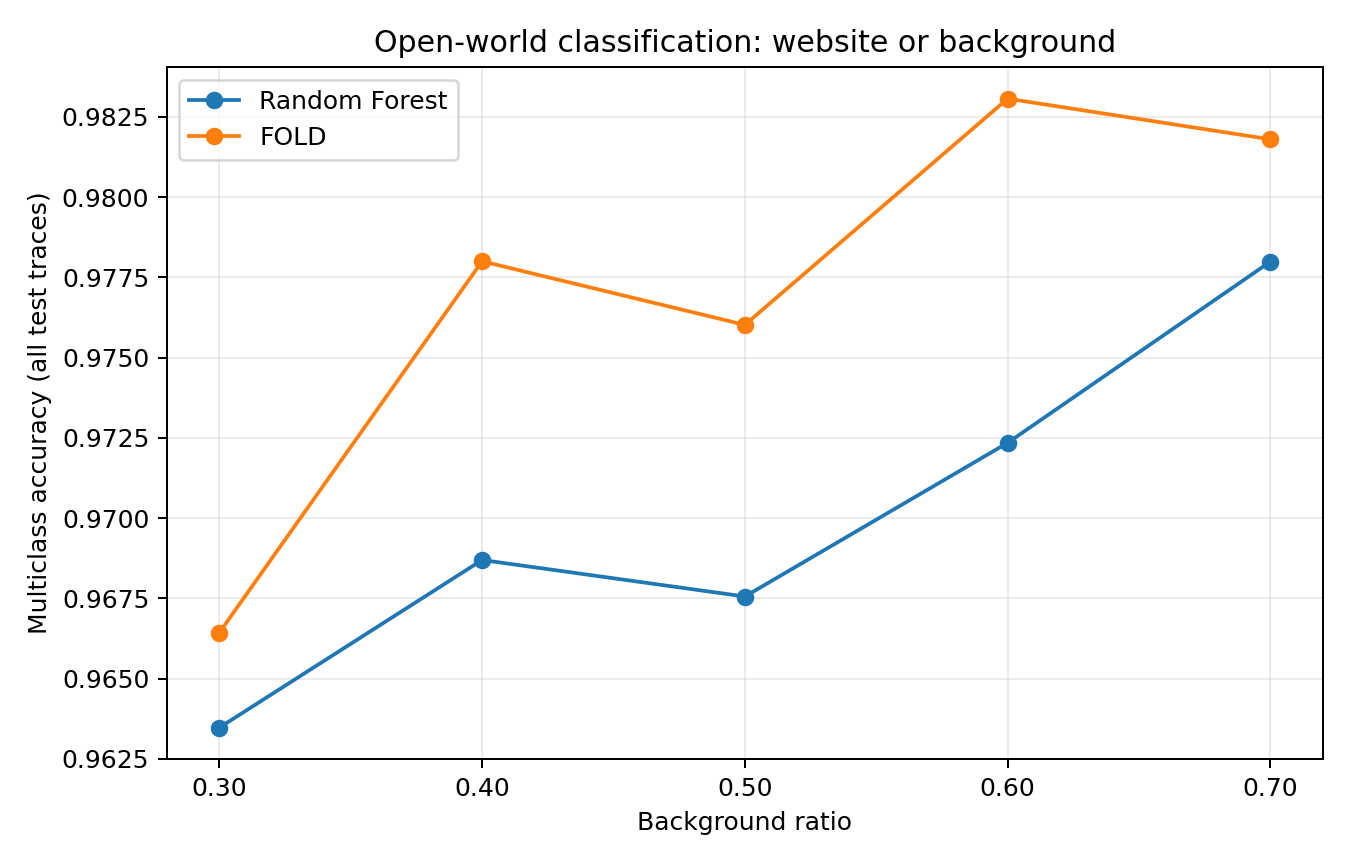
\includegraphics[width=\linewidth]{analysis/openworld_accuracy.png}
\caption{Accuracy sul test set.}\label{fig:open-accuracy}
\end{subfigure}\hfill
\begin{subfigure}{0.49\linewidth}
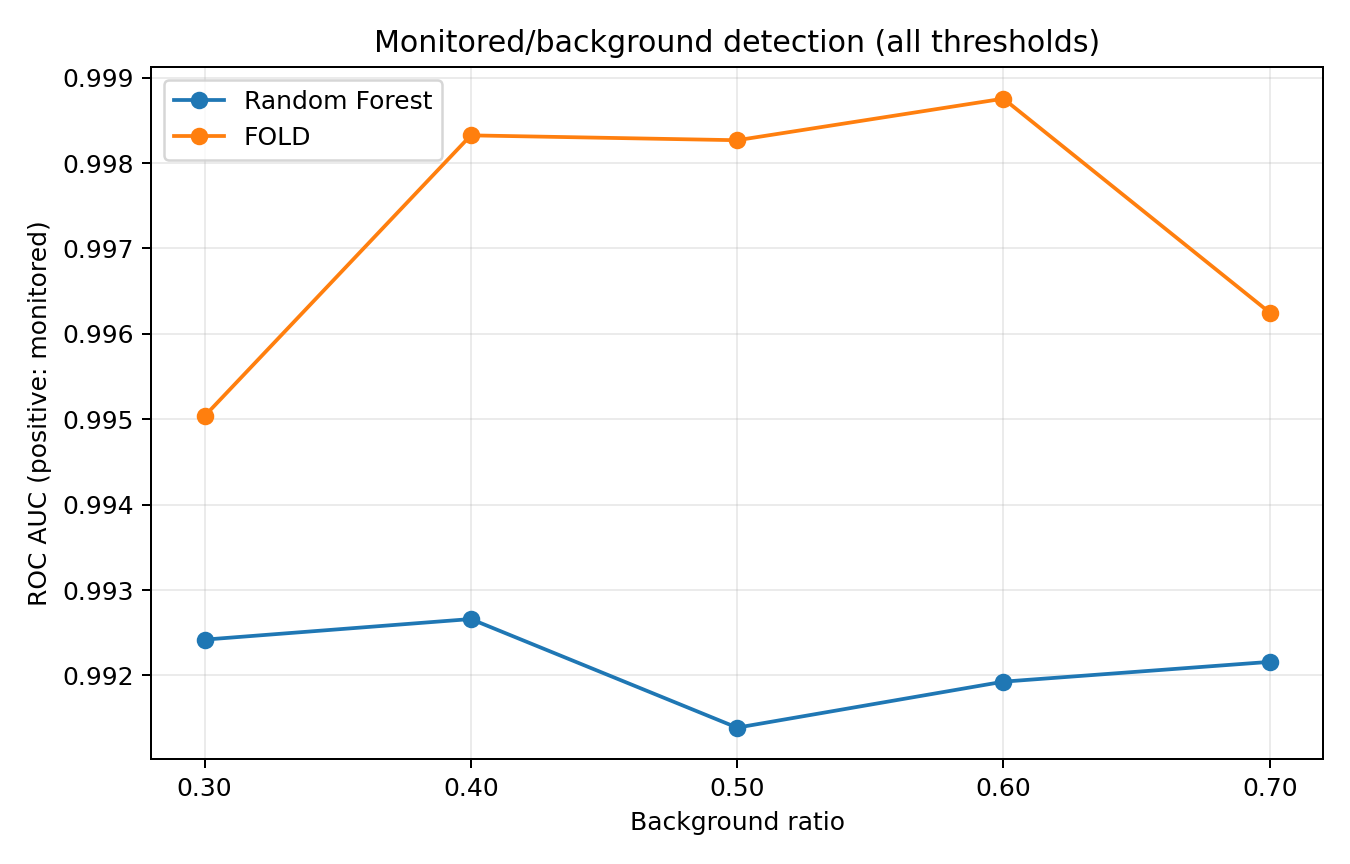
\includegraphics[width=\linewidth]{analysis/openworld_detection_auc.png}
\caption{ROC AUC monitored/background.}\label{fig:open-auc}
\end{subfigure}
\caption{Accuracy e ROC AUC di RF e FOLD nei cinque rapporti open-world, senza defense.}
\label{fig:open-performance}
\end{figure}

\subsection{Spiegazioni multiclass}
La Figura~\ref{fig:open-multi} e la Tabella~\ref{tab:open-multi-xai} non mostrano un andamento monotono evidente dei contributi al crescere del background. G1 e G2 sono i due gruppi con le attribuzioni medie assolute maggiori in tutti i rapporti; G2 supera G1 a 0.30 e 0.60.

La probabilità media Instagram varia tra 0.6257 e 0.8690, con il massimo a 0.50. I contributi medi con segno dei quattro gruppi sono positivi. Questi risultati riguardano le stesse 15 tracce Instagram nei cinque rapporti.

\begin{figure}[htbp]
\centering
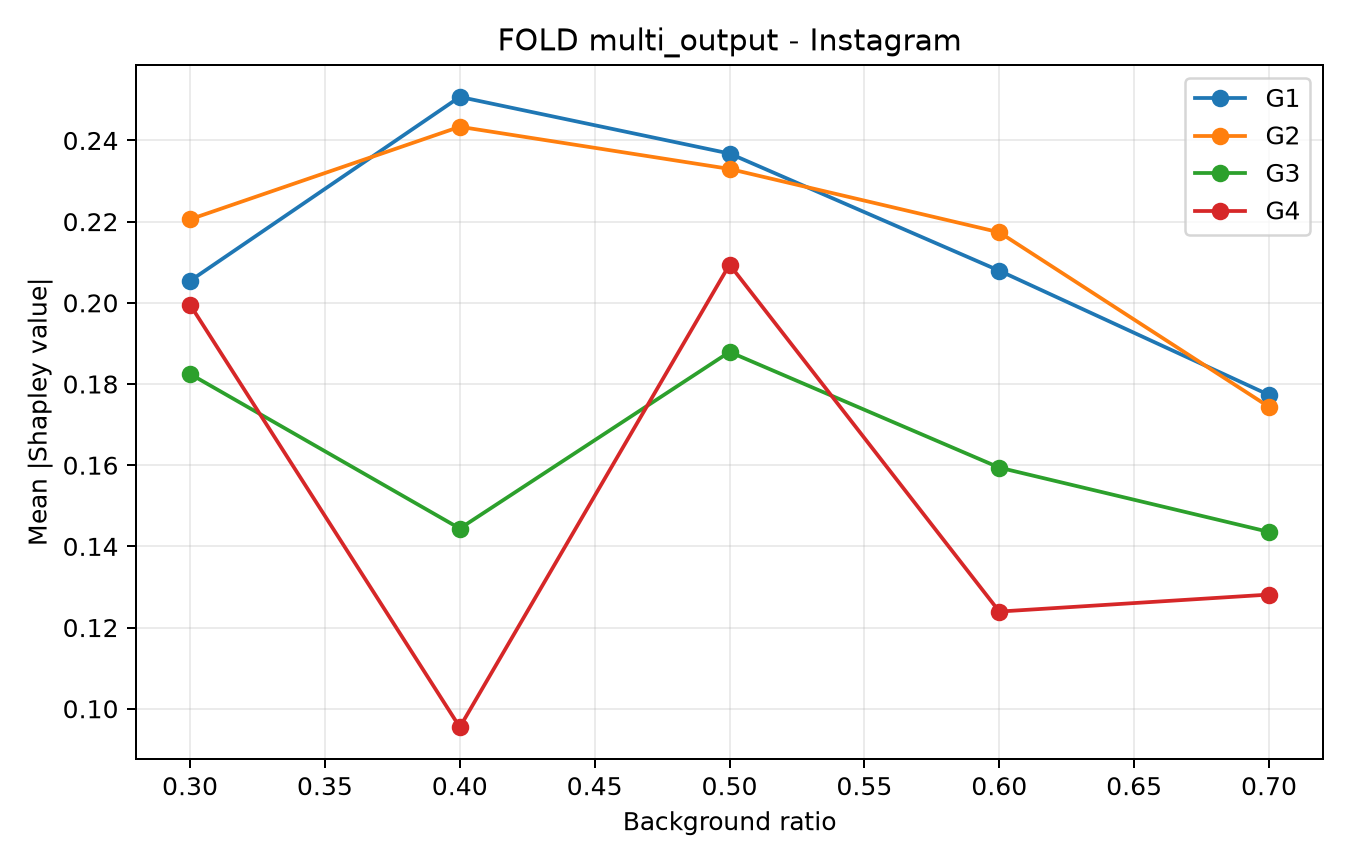
\includegraphics[width=0.86\linewidth]{analysis/openworld_multi_mean_abs_phi.png}
\caption{Contributi multiclass medi assoluti di FOLD sulle stesse 15 tracce Instagram nei cinque rapporti di background.}
\label{fig:open-multi}
\end{figure}

\subsection{Spiegazioni binary}
La Figura~\ref{fig:open-binary} mostra le magnitudini dei contributi per i cohort monitored e background. Le Tabelle~\ref{tab:open-binary-xai} e~\ref{tab:open-binary-signed} riportano probabilità, valori assoluti e valori con segno. La probabilità media delle reference miste è circa 0.5.

Nel cohort monitored i contributi medi sono positivi e aumentano quindi $P(\mathrm{monitored})$. G2 ha la magnitudine media maggiore in tutti i rapporti, seguito da G1 (Figura~\ref{fig:open-binary-monitored}). La probabilità media monitored supera 0.9995 in ogni rapporto. Il segno positivo della media non implica che ogni contributo individuale sia positivo.

Nel cohort background i contributi medi di tutti i gruppi sono negativi: diminuiscono $P(\mathrm{monitored})$ e spostano la predizione verso background. G1 ha la magnitudine media maggiore in tutti i rapporti (Figura~\ref{fig:open-binary-background}). La probabilità media monitored varia tra 0.0001 e 0.0677. I campioni background cambiano tra i rapporti: non si tratta dello stesso insieme di tracce confrontato cinque volte.

\begin{figure}[htbp]
\centering
\begin{subfigure}{0.86\linewidth}
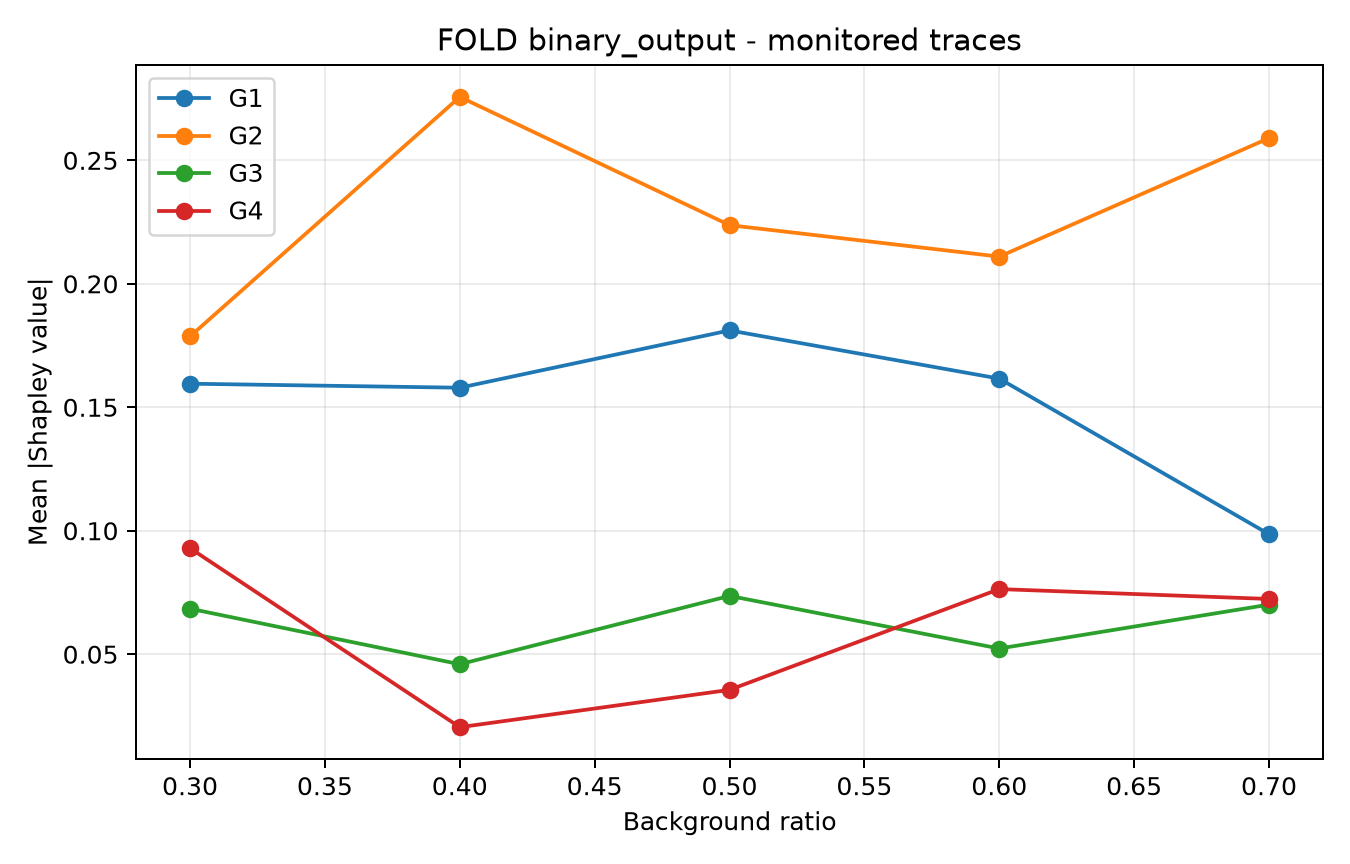
\includegraphics[width=\linewidth]{analysis/openworld_binary_monitored_mean_abs_phi.png}
\caption{Cohort monitored comune.}\label{fig:open-binary-monitored}
\end{subfigure}
\par\medskip
\begin{subfigure}{0.86\linewidth}
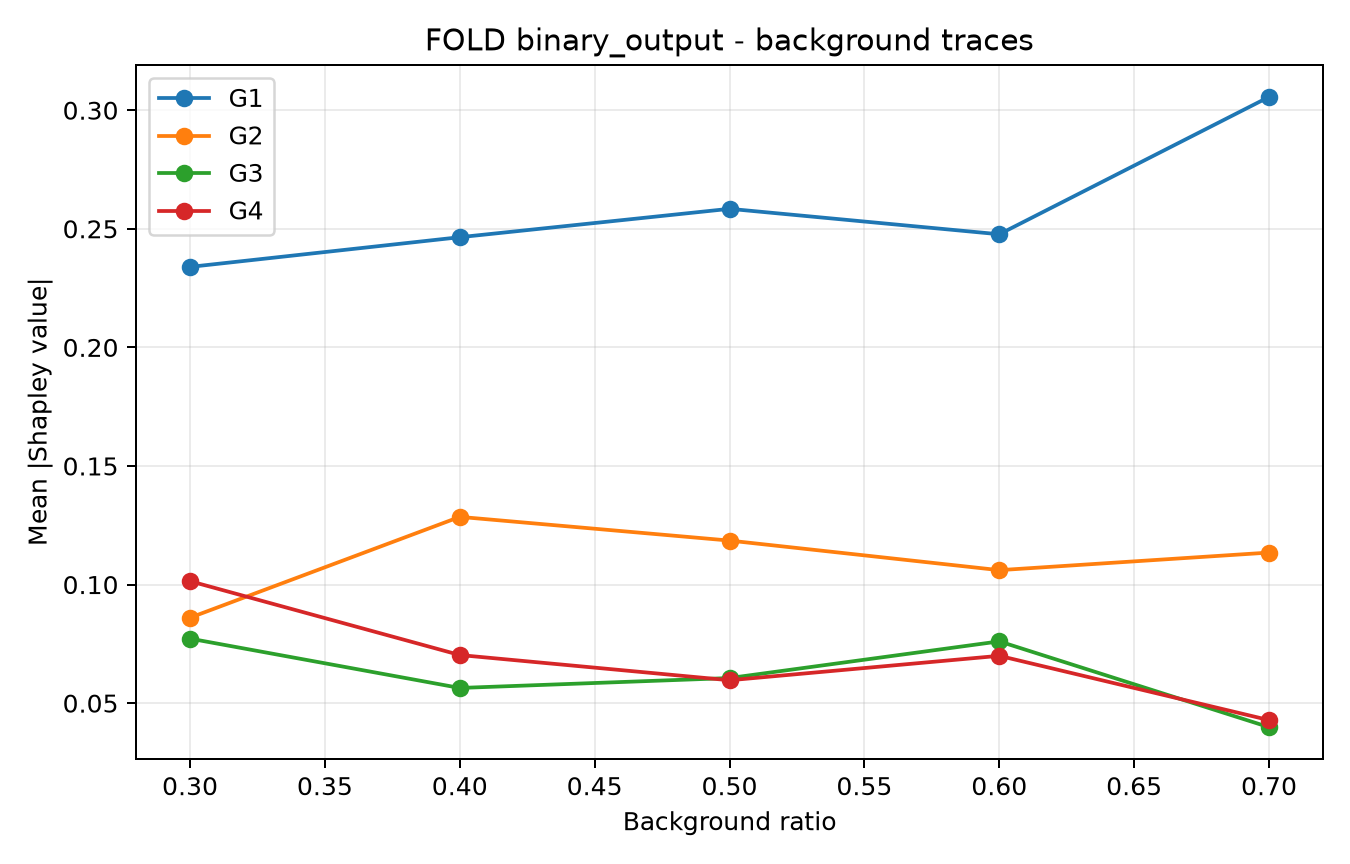
\includegraphics[width=\linewidth]{analysis/openworld_binary_background_mean_abs_phi.png}
\caption{Cohort background diversi tra i rapporti.}\label{fig:open-binary-background}
\end{subfigure}
\caption{Contributi binary medi assoluti di FOLD per 15 tracce monitored e 15 background, con 16 reference miste. I contributi con segno sono riportati nella Tabella~\ref{tab:open-binary-signed}.}
\label{fig:open-binary}
\end{figure}

\section{Limitazioni}
Per ogni configurazione è stata eseguita una sola ripetizione.I risultati non permettono quindi di valutare quanto le performance e le spiegazioni cambino ripetendo l'addestramento.

Le spiegazioni grouped dipendono dalle reference scelte. Con reference diverse potrebbero cambiare il riferimento di confronto e i contributi dei gruppi.

L'analisi multiclass dettagliata riguarda il cohort Instagram selezionato. Le osservazioni su questi campioni non possono essere estese automaticamente agli altri siti.

Nell'analisi binary i campioni background non sono gli stessi in tutti i rapporti. Le differenze osservate risentono quindi anche dei diversi insiemi di tracce spiegate.

\section{Conclusioni}
La pipeline implementata permette di spiegare sia la Random Forest, attraverso le sue feature, sia l'output finale di FOLD, attraverso gruppi di risoluzioni e un predictor end-to-end. Nella baseline i quattro gruppi non contribuiscono allo stesso modo sul cohort Instagram: G1 presenta il contributo medio assoluto maggiore, seguito da G2.

Le defense modificano performance e attribuzioni in modi diversi. Padding e combined producono le variazioni più evidenti nei risultati osservati, mentre dummy ha un impatto minore sulle performance nelle configurazioni testate. Fragmentation presenta una degradazione più moderata rispetto a padding e combined.

Nello scenario open-world FOLD mantiene buone performance nei cinque rapporti analizzati. Le spiegazioni binary mostrano contributi medi con direzione opposta nei due cohort: positivi per monitored e negativi per background. L'analisi permette così di distinguere i contributi alla probabilità di un sito da quelli alla decisione monitored/background.

\clearpage
\appendix
\section{Tabelle complete delle attribuzioni}
Le tabelle seguenti riportano le attribuzioni per tutte le configurazioni defense e open-world. Le Tabelle~\ref{tab:defense-xai} e~\ref{tab:open-multi-xai} riguardano l'output multiclass; le Tabelle~\ref{tab:open-binary-xai} e~\ref{tab:open-binary-signed} distinguono magnitudine e segno dei contributi binary. Probabilità e contributi sono arrotondati a quattro decimali.

\begin{table}[htbp]
\centering\small
\caption{Risultati multiclass completi della baseline e delle defense sulle stesse 15 tracce Instagram. $\overline{P}_8$ è la probabilità media Instagram; G1--G4 riportano i contributi medi assoluti.}
\label{tab:defense-xai}
\begin{tabular}{lrrrrrr}
\toprule
Defense & Intensità & $\overline{P}_8$ & G1 & G2 & G3 & G4 \\
\midrule
Baseline & 0.00 & 0.8451 & 0.2950 & 0.2146 & 0.1654 & 0.1687 \\
Padding & 0.10 & 0.9250 & 0.2829 & 0.2136 & 0.2169 & 0.2103 \\
Padding & 0.30 & 0.8659 & 0.2741 & 0.2451 & 0.1685 & 0.1770 \\
Padding & 0.50 & 0.5052 & 0.1434 & 0.1247 & 0.1383 & 0.0981 \\
Padding & 0.70 & 0.1479 & 0.0415 & 0.0354 & 0.0377 & 0.0397 \\
Padding & 1.00 & 0.0262 & 0.0059 & 0.0041 & 0.0078 & 0.0048 \\
Dummy & 0.10 & 0.7965 & 0.2787 & 0.1772 & 0.1541 & 0.1857 \\
Dummy & 0.30 & 0.8280 & 0.3245 & 0.2106 & 0.1407 & 0.1504 \\
Dummy & 0.50 & 0.9137 & 0.3035 & 0.2031 & 0.1783 & 0.2279 \\
Dummy & 0.70 & 0.8087 & 0.2860 & 0.2125 & 0.1662 & 0.1431 \\
Dummy & 1.00 & 0.8214 & 0.2593 & 0.1902 & 0.2130 & 0.1576 \\
Fragmentation & 0.10 & 0.8463 & 0.2960 & 0.2098 & 0.1592 & 0.1804 \\
Fragmentation & 0.30 & 0.8592 & 0.2644 & 0.2296 & 0.1692 & 0.1948 \\
Fragmentation & 0.50 & 0.6807 & 0.2094 & 0.1626 & 0.1515 & 0.1627 \\
Fragmentation & 0.70 & 0.8291 & 0.2396 & 0.2190 & 0.1779 & 0.1900 \\
Fragmentation & 1.00 & 0.8373 & 0.2362 & 0.1960 & 0.1963 & 0.2074 \\
Combined & 0.10 & 0.8410 & 0.1969 & 0.1941 & 0.2219 & 0.2271 \\
Combined & 0.30 & 0.4606 & 0.1121 & 0.1077 & 0.1201 & 0.1251 \\
Combined & 0.50 & 0.0659 & 0.0217 & 0.0136 & 0.0138 & 0.0136 \\
Combined & 0.70 & 0.0393 & 0.0141 & 0.0074 & 0.0085 & 0.0084 \\
Combined & 1.00 & 0.2256 & 0.0633 & 0.0489 & 0.0539 & 0.0590 \\
\bottomrule
\end{tabular}
\end{table}

\begin{table}[htbp]
\centering\small
\caption{Risultati multiclass open-world sul cohort Instagram. $\overline{P}_8$ è la probabilità media Instagram; G1--G4 riportano i contributi medi assoluti.}
\label{tab:open-multi-xai}
\begin{tabular}{rrrrrr}
\toprule
Background & $\overline{P}_8$ & G1 & G2 & G3 & G4 \\
\midrule
0.30 & 0.8103 & 0.2054 & 0.2206 & 0.1825 & 0.1995 \\
0.40 & 0.7364 & 0.2507 & 0.2434 & 0.1444 & 0.0955 \\
0.50 & 0.8690 & 0.2368 & 0.2330 & 0.1879 & 0.2094 \\
0.60 & 0.7120 & 0.2079 & 0.2174 & 0.1594 & 0.1239 \\
0.70 & 0.6257 & 0.1773 & 0.1744 & 0.1436 & 0.1281 \\
\bottomrule
\end{tabular}
\end{table}

\begin{table}[htbp]
\centering\small
\caption{Risultati binary per 15 campioni di ciascun cohort e rapporto. $\overline{P}_{M}$ è la media di $P(\mathrm{monitored})$; G1--G4 riportano i contributi medi assoluti.}
\label{tab:open-binary-xai}
\begin{tabular}{rlrrrrr}
\toprule
Background & Cohort & $\overline{P}_{M}$ & G1 & G2 & G3 & G4 \\
\midrule
0.30 & Monitored & 0.9996 & 0.1595 & 0.1787 & 0.0684 & 0.0929 \\
0.30 & Background & 0.0059 & 0.2339 & 0.0860 & 0.0772 & 0.1014 \\
0.40 & Monitored & 1.0000 & 0.1579 & 0.2757 & 0.0459 & 0.0205 \\
0.40 & Background & 0.0677 & 0.2465 & 0.1285 & 0.0564 & 0.0703 \\
0.50 & Monitored & 1.0000 & 0.1811 & 0.2237 & 0.0736 & 0.0356 \\
0.50 & Background & 0.0425 & 0.2584 & 0.1185 & 0.0606 & 0.0597 \\
0.60 & Monitored & 1.0000 & 0.1616 & 0.2110 & 0.0523 & 0.0764 \\
0.60 & Background & 0.0002 & 0.2477 & 0.1061 & 0.0760 & 0.0700 \\
0.70 & Monitored & 1.0000 & 0.0986 & 0.2590 & 0.0701 & 0.0724 \\
0.70 & Background & 0.0001 & 0.3056 & 0.1135 & 0.0399 & 0.0428 \\
\bottomrule
\end{tabular}
\end{table}

\begin{table}[htbp]
\centering\small
\caption{Contributi binary medi con segno. Valori positivi aumentano $P(\mathrm{monitored})$ rispetto alle reference; valori negativi la diminuiscono.}
\label{tab:open-binary-signed}
\begin{tabular}{rlrrrr}
\toprule
Background & Cohort & G1 & G2 & G3 & G4 \\
\midrule
0.30 & Monitored & 0.1595 & 0.1787 & 0.0684 & 0.0929 \\
0.30 & Background & -0.2339 & -0.0860 & -0.0727 & -0.1014 \\
0.40 & Monitored & 0.1579 & 0.2757 & 0.0459 & 0.0205 \\
0.40 & Background & -0.2022 & -0.1285 & -0.0404 & -0.0612 \\
0.50 & Monitored & 0.1811 & 0.2096 & 0.0736 & 0.0356 \\
0.50 & Background & -0.2584 & -0.1185 & -0.0343 & -0.0464 \\
0.60 & Monitored & 0.1616 & 0.2097 & 0.0523 & 0.0764 \\
0.60 & Background & -0.2477 & -0.1061 & -0.0760 & -0.0700 \\
0.70 & Monitored & 0.0986 & 0.2590 & 0.0701 & 0.0724 \\
0.70 & Background & -0.3056 & -0.1135 & -0.0399 & -0.0408 \\
\bottomrule
\end{tabular}
\end{table}

\end{document}
